\chapter{Blockchain \& Bitcoin}

\section{Introduzione}

\subsection{Blockchain}

La \textit{blockchain} (letteralmente "catena di blocchi") è una struttura dati
\textbf{condivisa} e "\textbf{immutabile}". È definita come un \textit{registro
    digitale} le cui voci sono raggruppate in "\textbf{blocchi}", concatenati in
ordine cronologico, e la cui integrità è garantita dall'uso della
\textbf{crittografia}. Sebbene la sua dimensione sia destinata a crescere nel
tempo, è immutabile in quanto, di norma, il suo contenuto una volta scritto non
è più né modificabile né eliminabile, a meno di non invalidare l'intera
struttura. Tali tecnologie sono incluse nella più ampia famiglia delle
“\textit{Distributed Ledger}”, ossia sistemi che si basano su un registro
distribuito, che può essere letto e modificato da più nodi di una rete. Non è
richiesto che i nodi coinvolti conoscano l'identità reciproca o si fidino l'uno
dell'altro. Difatti, per garantire la coerenza tra le varie copie, l'aggiunta di
un nuovo blocco è globalmente regolata da un protocollo condiviso. Una volta
autorizzata l'aggiunta del nuovo blocco, ogni nodo aggiorna la propria copia
privata: la natura stessa della struttura dati garantisce l'assenza di una sua
manipolazione futura. Le caratteristiche che accomunano i sistemi sviluppati con
le tecnologie Blockchain e Distributed Ledger sono digitalizzazione dei dati,
\textbf{decentralizzazione}, \textbf{disintermediazione}, \textbf{tracciabilità
    dei trasferimenti}, \textbf{trasparenza}/verificabilità, \textbf{immutabilità}
del registro e programmabilità dei trasferimenti. La natura distribuita e il
modello cooperativo rendono robusto e sicuro il processo di validazione, ma
presentano tempi non trascurabili, dovuti in gran parte al processo di
validazione dei blocchi e alla sincronizzazione delle rete. L'autenticazione
avviene tramite collaborazione di massa ed è alimentata da interessi collettivi.
L'utilizzo di questa tecnologia consente anche di superare il problema
dell'infinita riproducibilità di un bene digitale e della doppia spesa, senza
l'utilizzo di un server centrale o di un'autorità. Talvolta risulta possibile
che alcuni nodi della rete producano simultaneamente più blocchi "concorrenti"
(ossia collegati a uno stesso blocco già esistente, ma diversi tra loro nel
contenuto): ciò dà origine a una biforcazione (fork) nella catena. Il protocollo
di aggiornamento specifica quale regola i nodi debbano adottare per selezionare
il blocco da accettare, tra quelli concorrenti. I blocchi non selezionati per
l'inclusione nella catena sono chiamati "\textit{blocchi orfani}".

\begin{figure}[H]
    \centering
    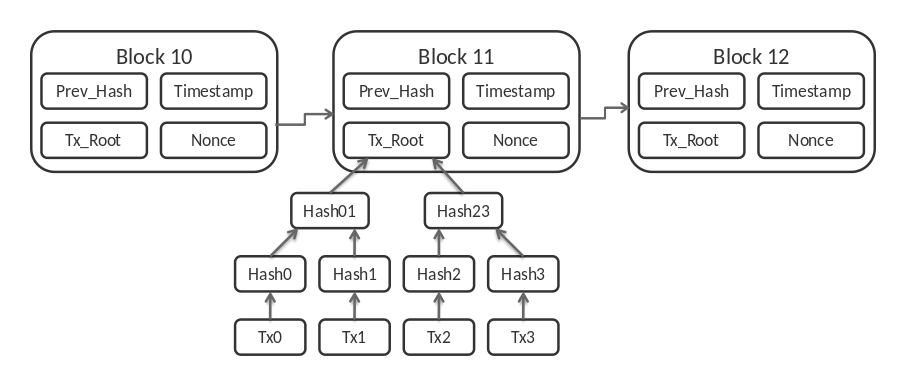
\includegraphics[width=\textwidth, keepaspectratio]{capitoli/bitcoin/imgs/bit1.png}
    \caption{Esempio di blocchi e del loro contenuto all'interno della Blockchain.}
\end{figure}

\subsection{Bitcoin}

Il bitcoin si comporta più come “\textit{oro}” che come “moneta” perché il
valore cambia nel tempo. Più che proprietà o possesso di bitcoin/monete si parla
di \textit{diritto di spesa}, che si ottiene conoscendo una determinata chiave
di cifratura. Si possono inviare e ricevere bitcoin sfruttando una exchange
platform che consente l'invio di denaro utilizzando un sistema a doppia chiave.
In sostanza, il passaggio di possesso di bitcoin avviene cambiando l'utente che
è a conoscenza della chiave che è in grado di decriptarli. Questo passaggio di
chiavi viene fatto dall'exchange platform. Quindi si genera una coppia chiave
pubblica-privata, si divulga la pubblica e si ottengono i bitcoin sopra che poi
con la chiava privata potranno essere spesi o ceduti ad un altro utente.

\begin{figure}[H]
    \centering
    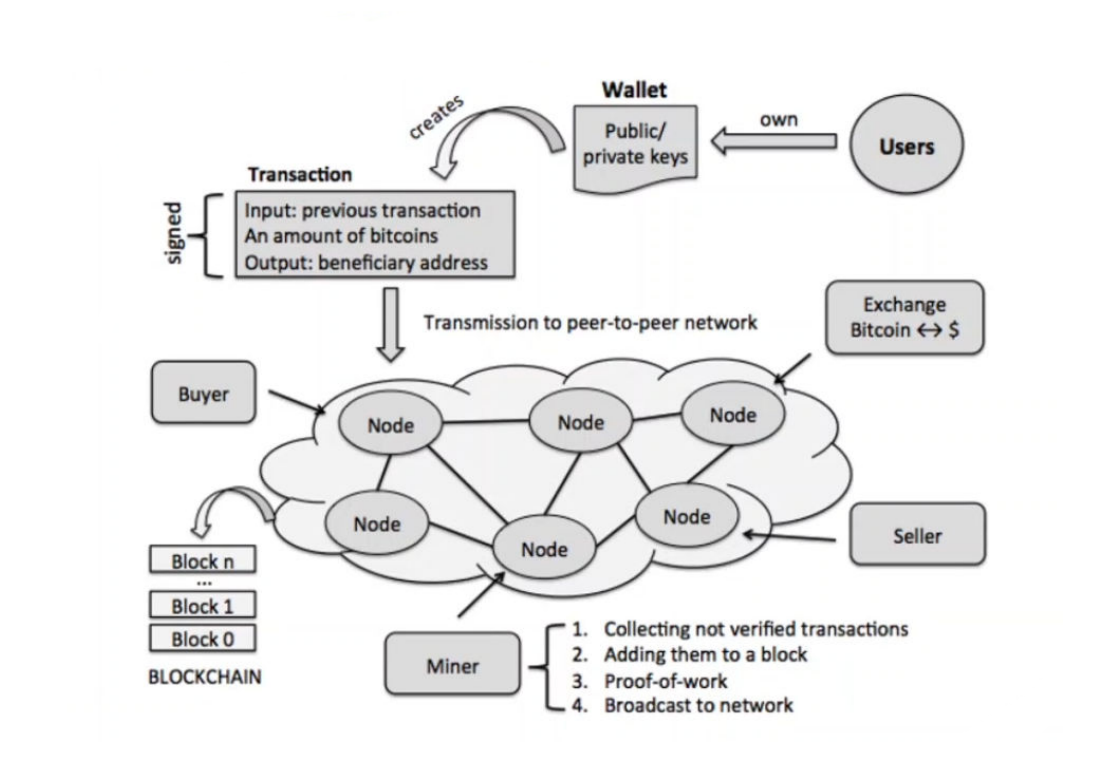
\includegraphics[width=14cm, keepaspectratio]{capitoli/bitcoin/imgs/bit2.png}
    \caption{Immagine raffigurante l'ecosistema Bitcoin.}
\end{figure}

Nella precedente immagine possiamo distinguere:

\begin{itemize}
    \item \textbf{Exchange}: trasformazione bitcoin e moneta,
    \item \textbf{Nodi} per registrare transazioni,
    \item Gli \textbf{utenti} che voglio partecipare all'ecosistema devo essere
          dotati di un Wallet,
    \item Un \textbf{wallet} è un software che permette
          di gestire in maniera facile le copie di chiavi private-pubbliche, che
          servono per ricevere o dare diritti di spesa/transazioni,
    \item Le \textbf{transazioni} vengono salvate sui database distribuiti e
          vengono replicate su tutti i nodi della rete.
\end{itemize}

\subsubsection{Bitcoin Core}

Il software Bitcoin Core\footnote{In inglese Bitcoin Core
    \emoji{upside-down-face}} (evoluzione Bitcoin-Qt) può essere scaricato come
qualsiasi altro programma sul nostro computer. Bitcoin Core implementa tutti
gli aspetti della rete Bitcoin, quindi scaricarlo ti renderà un nodo
completo della rete, ciò include una copia esatta e completa di tutte le
operazioni che sono state effettuate con Bitcoin dal suo lancio nel 2009.
Naturalmente sarà costantemente aggiornato, quindi la richiesta di spazio di
archiviazione disponibile sul disco rigido sarà di almeno 400 GB.

\subsubsection{Bitcoin Actors}

Possiamo distinguere diverse tipologie di nodi in base alle funzioni che
implementano:

\begin{figure}[H]
    \centering
    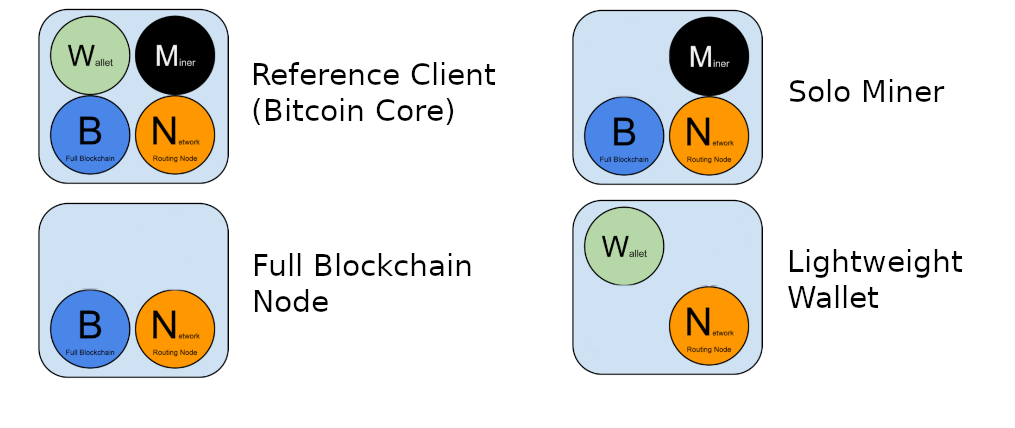
\includegraphics[width=15cm, keepaspectratio]{capitoli/bitcoin/imgs/bit33.png}
\end{figure}

\begin{itemize}
    \item \textit{Wallet} (verde): mantiene le chiavi pubbliche e private.
    \item Routing (arancione): quando riceve una transazione può fare il
          broadcast in modo da comunicarlo a tutti.
    \item \textit{Full blockchain} (blu): tiene il database di tutte le transazioni fatte
          e/o può creare transazioni
    \item \textit{Miner} (nero): in genere le transazioni da inserire su un blocco sono
          tantissime, il miner ha il compito di selezionarle e metterle in un
          blocco (nelle blockchain si può inserire solo un blocco di transazioni
          per volta, e non una transazione alla volta ), per poi comunicare le
          operazioni portate a termine agli altri nodi in modo che tutti
          aggiornino le informazioni.
\end{itemize}

\subsubsection{Miner}

Tutte le transazioni che devono essere ancora inserite nella blockchain
richiedono di essere validate dai mainer e mentre sono in attesa risiedono in un
pool generale. Sono i \textbf{Miner} a decidere quale transazione mettere in un
blocco. In generale vengono inserite prima le transazioni con importo maggiore o
quelle più vecchie, ma è possibile pagare una piccola commissione al miner per
far salire la propria transazione di priorità. Inoltre come compenso aggiuntivo
nel protocollo è stabilito che quando i miner inseriscono nuove transazioni
ricevono un compenso in nuovi bitcoin (creati dal nulla). Questi compenso in
bitcoin tuttavia è ideato per diminuire nel tempo fino a raggiungere
eventualmente uno zero in base al rapporto compenso/numero di blocchi inseriti.
Tutto ciò avviene affinché i miner si concentrino principalmente sulle
transazioni (dove riceveranno le commissioni degli utenti) e non
sull'inserimento di nuove monete/blocchi. Se così non fosse non sarebbero
incentivati e l'ecosistema bitcoin crollerebbe.
Per regolare queste operazioni di validazione delle transazioni esistono vari
protocolli, i più comuni nell'ambito delle criptovalute sono il \textbf{Proof of
    Work} e il \textbf{Proof of Stake}.

\paragraph{PoW:}
nel proof of work la ricompensa non viene data a tutti i nodi ma al primo che
riesce a risolvere un problema crittografico, questo si aggiudicherà il diritto
di scegliere quale transazione inserire nel blocco. Per risolvere il problema il
miner dovrà trovare una stringa che aggiunta alle transazioni del blocco dia
come risultato \verb|00000xxxxxxxxxxx| una volta hashata. L'unico modo per
ottenere la stringa è facendo dei tentativi per indovinarla. Una volta
verificata la correttezza della stringa dagli altri nodi l'operazione sarà
approvata. La difficoltà per i miner varia in base al numero di \verb|0|
iniziali contenuti nella stringa finale, questi \verb|0| possono essere
aumentati o diminuiti in base al tempo di risoluzione medio impiegato dai miner
(che dovrebbe sempre aggirarsi intorno ai 10 minuti). Infine, prima di
aggiungere definitivamente il blocco, viene inserita una transazione fittizia in
più, chiamata \textbf{Coinbase}, dove viene registrato il fatto che il miner riceve
il suo compenso di nuovi bitcoin.

\subsubsection{Escrow Contracts}

Questi sono un particolare tipo di smart contract basato su Bitcoin in cui per
trasferire una somma di denaro da A a B ci si appoggia ad una terza entità in
cui viene depositato il compenso del contratto che verrà rilasciato solo quando
le condizioni definite in precedenza verranno soddisfatte.

\begin{figure}[H]
    \centering
    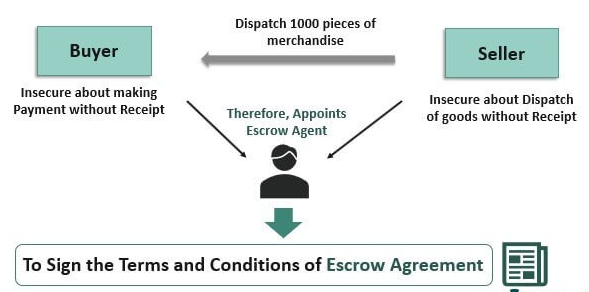
\includegraphics[width=10cm, keepaspectratio]{capitoli/bitcoin/imgs/escort.png}
\end{figure}


\section{Sicurezza e Blockchain}

\subsection{Double Spending}

È un potenziale attacco in cui un bitcoin viene inviato a 2 persone
contemporaneamente, benché non sia realizzabile nella blockchain di bitcoin
poiché è intrinsecamente resistente fa da base per molti altri attacchi e dunque
spiegheremmo brevemente come funziona. Un miner A invia denaro a due utenti B e
C contemporaneamente, di norma in bitcoin viene approvata la prima transazione
(dato che ci si basa sull'hash e sul timestamp) ma supponiamo che entrambe
vengano approvate in contemporanea su due blocchi diversi, allora entrambe
verranno viste come transazioni valide e ci sarà una possibile fork della
blockchain. In bitcoin però prima o poi una delle due blockchain
risulterà essere più lunga dell'altra e verrà presa quella come blockchain
valida e perciò una delle due transazioni verrà rifiutata.

\subsubsection{51\% Attack}

Un possibile attacco che concettualmente è simile a quello del double spending è
quello del 51\% in cui un utente che dispone di un ampia porzione di potenza di
calcolo della rete può tentare di manipolare la blockchain portando avanti in
segreto una copia alterata della stessa. Se il miner che sta portando avanti
questo attacco riesce a generare una blockchain più lunga di quella vera allora
per la regola della catena più lunga, divulgandola la farà accettare dalla rete
e diventerà dunque la vera blockchain.\\
Per imporre i suoi blocchi, un'organizzazione dovrebbe controllare il 51\% dei
nodi (è detto 51\% attack), per avere potenza di calcolo sufficiente a produrre
(con buona probabilità) catene di blocchi lunghe prima di tutti gli altri nodi,
ciò è altamente improbabile. Non è possibile che questo attacco abbia successo
perché nessuno dispone di una potenza di calcolo così elevata.

\subsection{Wallet attack}

Ti vengono rubate le credenziali di accesso al wallet o le chiavi private
\emoji{man-dark-skin-tone}.

\subsection{Transaction Malleability }

Gli attacchi di malleability consistono nello sfruttare la manipolabilità
dell'id delle transazioni che viene calcolato con un hash. Andando a cambiare
l'id della transazione si verificherà un effetto a cascata causato dall'hash e
dunque il mittente della transazione non la riconoscerà più come propria anche
se c'è la possibilità che i soldi vengano comunque inviati. Cosi facendo
l'utente malevolo ha un pretesto per richiedere nuovamente i soldi alla vittima
affermando che non ha mai inviato i soldi.

\subsection{Sybil Attack}

Un Sybil attack è un attacco in cui un utente o un gruppo di utenti prende il
controllo della rete creando un elevato numero di nuovi account e nodi, avendo
così la maggioranza dei nodi. Questo consentirebbe di poter far approvare dei
blocchi con transazioni fraudolente. Tutto ciò risulta essere impossibile dato
che viene mitigato dalla PoW.
